\documentclass[11pt, tikz, border=10pt]{standalone}
\usepackage{pgfplots}
\pgfplotsset{compat=1.18}
\usepackage{amsmath}
\usetikzlibrary{calc, arrows.meta, positioning, shapes.geometric, fit, patterns}

\definecolor{bglight}{HTML}{F8FAFC}
\definecolor{borderc}{HTML}{E2E8F0}
\definecolor{textmain}{HTML}{0F172A}
\definecolor{textsub}{HTML}{475569}
\definecolor{chartblue}{HTML}{0284C7}
\definecolor{queryred}{HTML}{EF4444}
\definecolor{valleygreen}{RGB}{35,95,25}
\definecolor{customorange}{RGB}{255,130,0}

\begin{document}

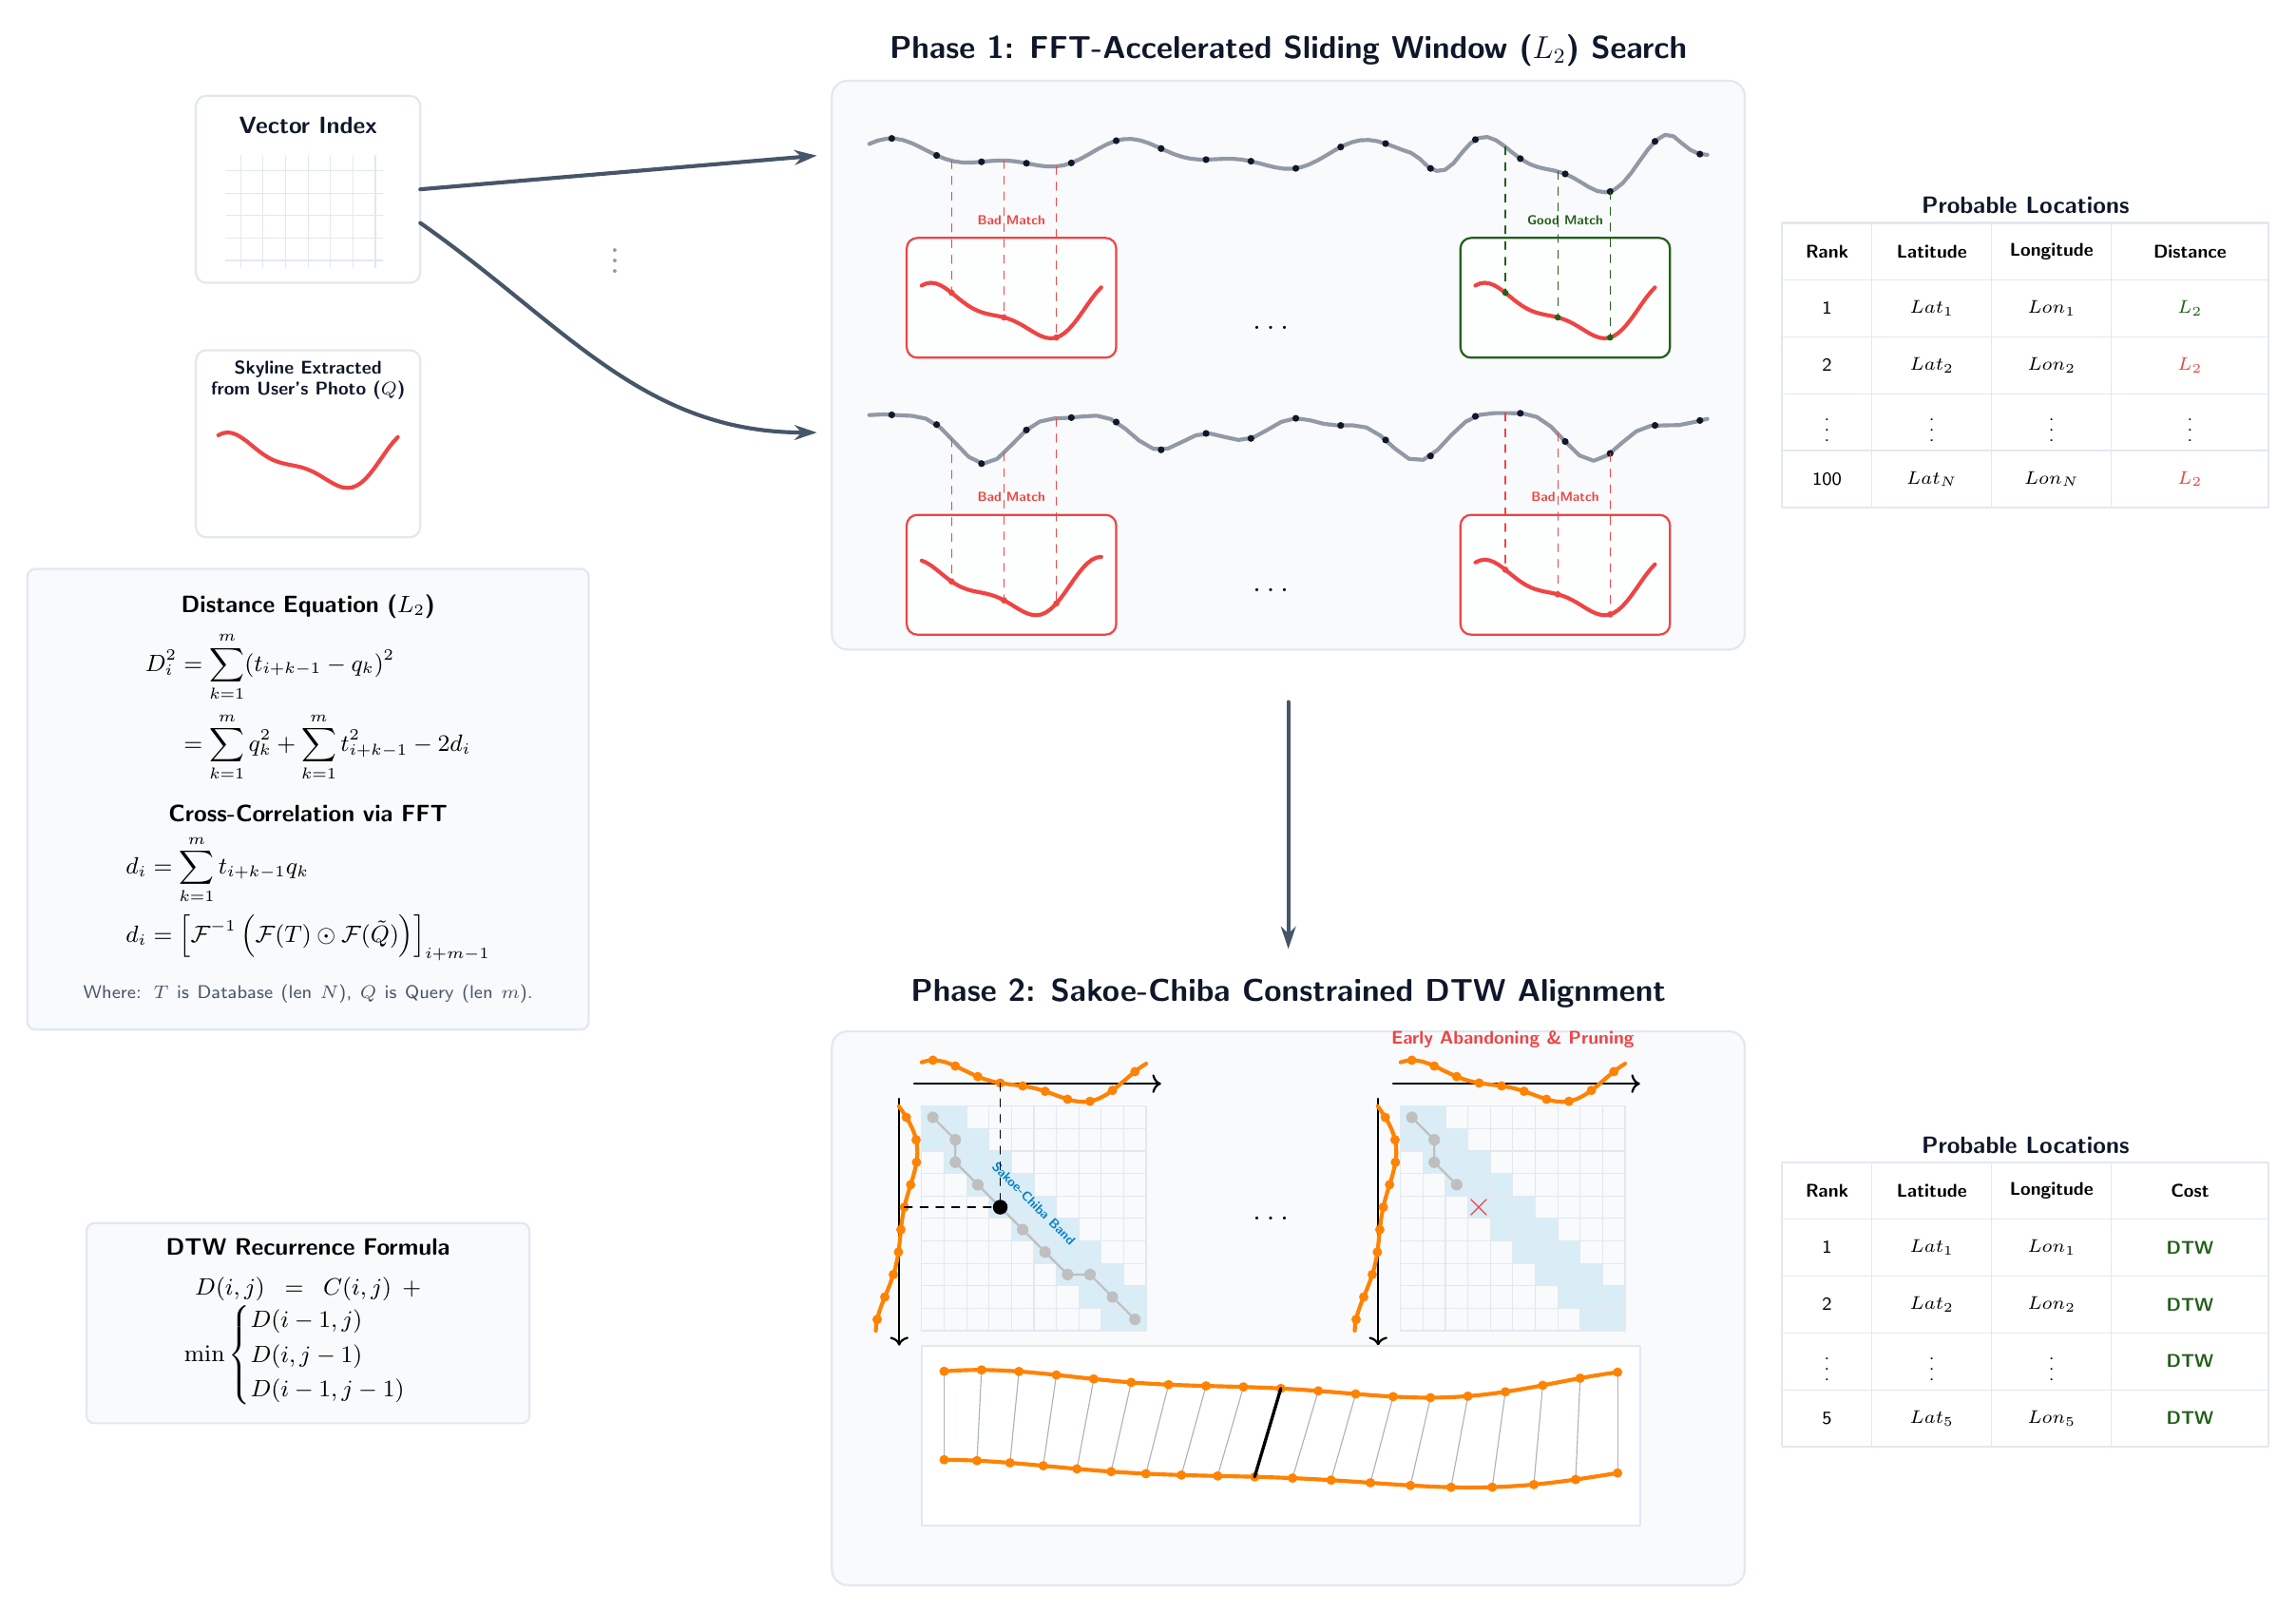
\begin{tikzpicture}[
    line join=round, 
    line cap=round,
    declare function={
        % Linear interpolation step (100% numerically stable, zero risk of TeX overflow)
        sstep(\x,\a,\b) = (\x < \a ? 0 : (\x > \b ? 1 : (\x - \a)/(\b - \a)));
        % Exact mathematical formula from page2.tex representing the user's skyline
        user_skyline(\x) = 0.35 + 0.20*sin(\x*200 + 45) + 0.08*cos(\x*380);
        % Base Curve 1 components (matching the 1.6 scale centered at 8.6 with new vertical offset)
        target_match(\x) = 5.90 + 1.6 * user_skyline((\x - 8.6) * 0.75);
        target_noise(\x) = 6.6 + 0.15*sin(\x*110) - 0.08*cos(\x*230);
        % Unified single continuous function with smooth transitions
        base_curve_one(\x) = (\x < 7.8 ? target_noise(\x) : (\x < 8.4 ? (1.0 - sstep(\x, 7.8, 8.4))*target_noise(\x) + sstep(\x, 7.8, 8.4)*target_match(\x) : (\x < 11.2 ? target_match(\x) : (\x < 11.7 ? (1.0 - sstep(\x, 11.2, 11.7))*target_match(\x) + sstep(\x, 11.2, 11.7)*target_noise(\x) : target_noise(\x) ))));
        % DTW Wave-form signals for the axes (derived from the real user's skyline)
        tsine(\x) = 1.2 * user_skyline(\x * 0.6) - 0.4;
        lsine(\x) = 1.2 * user_skyline(\x * 0.5 + 0.1) - 0.4;
    },
    headerstyle/.style={font=\large\sffamily\bfseries, text=textmain},
    substyle/.style={font=\small\sffamily\bfseries, text=textsub},
    boxstyle/.style={draw=borderc, thick, fill=white, rounded corners=4pt, inner sep=6pt, align=center},
    mathstyle/.style={draw=borderc, thick, fill=bglight, rounded corners=3pt, inner sep=6pt, align=center, font=\sffamily\small},
    arrowstyle/.style={-{Stealth[length=3mm, width=2mm]}, line width=1.5pt, draw=textsub}
]

    % ========================================================
    % 1. PHASE 1: VECTOR INDEX GRID & SLIDING WINDOW SEARCH
    % ========================================================
    \node[headerstyle] (title1) at (9.6, 13.2) {Phase 1: FFT-Accelerated Sliding Window ($L_2$) Search};
    
    % Vector Index Grid
    \begin{scope}[shift={(-5.0, 10.1)}]
        \draw[borderc, thick, fill=white, rounded corners=4pt] (0,0) rectangle (3.0,2.5);
        \node[font=\sffamily\bfseries\small, text=textmain] at (1.5, 2.1) {Vector Index};
        \draw[borderc, thin, step=0.3cm] (0.4,0.2) grid (2.5,1.7);
    \end{scope}

    % Skyline Extracted Box
    \begin{scope}[shift={(-5.0, 6.7)}]
        \draw[borderc, thick, fill=white, rounded corners=4pt] (0,0) rectangle (3.0,2.5);
        \node[font=\sffamily\bfseries\scriptsize, text=textmain, align=center] at (1.5, 2.1) {Skyline Extracted\\from User's Photo ($Q$)};
        % Exact page2.tex curve scaled to fit the display bounds beautifully
        \draw[queryred, line width=1.5pt] plot[domain=0.3:2.7, samples=40] (\x, {0.45 + 1.6*user_skyline((\x-0.3)*0.75)});
    \end{scope}

    % Mathematical Formula Box with clean, spacious derivation
    \node[mathstyle, text width=6.8cm, inner sep=10pt] (p1math) at (-3.5, 3.2) {
        \textbf{Distance Equation ($L_2$)}\\
        \vspace{4pt}
        $\begin{aligned}
            D_i^2 &= \sum_{k=1}^{m} (t_{i+k-1} - q_k)^2 \\
                  &= \sum_{k=1}^{m} q_k^2 + \sum_{k=1}^{m} t_{i+k-1}^2 - 2 d_i
        \end{aligned}$\\
        \vspace{8pt}
        \textbf{Cross-Correlation via FFT}\\
        \vspace{4pt}
        $\begin{aligned}
            d_i &= \sum_{k=1}^{m} t_{i+k-1} q_k \\
            d_i &= \left[\mathcal{F}^{-1}\left(\mathcal{F}(T) \odot \mathcal{F}(\tilde{Q})\right)\right]_{i+m-1}
        \end{aligned}$\\
        \vspace{8pt}
        \scriptsize\color{textsub} Where: $T$ is Database (len $N$), $Q$ is Query (len $m$).
    };

    % Sliding Window Curves Panel with expanded vertical padding (Height = 7.6)
    \begin{scope}[shift={(3.5, 5.2)}]
        % Background panel
        \draw[borderc, thick, fill=bglight, rounded corners=6pt] (0.0, 0.0) rectangle (12.2, 7.6);
        
        % ----------------------------------------------------
        % ROW 1: BASE CURVE 1 (Single continuous C1-smooth curve)
        % ----------------------------------------------------
        \draw[textsub!60, line width=1.5pt] plot[domain=0.5:11.7, samples=100] (\x, {base_curve_one(\x)});
        
        % Discrete dots perfectly aligned along the continuous curve
        \foreach \xd in {0.8,1.4,...,11.6} { 
            \fill[textmain] (\xd, {base_curve_one(\xd)}) circle (1.3pt); 
        }

        % ----------------------------------------------------
        % ROW 2: SLIDING WINDOWS (Under Base Curve 1)
        % ----------------------------------------------------
        % Window W_11 (Bad Match - Left)
        \draw[queryred, thick, rounded corners=4pt, fill=white, fill opacity=0.85] (1.0, 3.9) rectangle (3.8, 5.5);
        \node[font=\sffamily\tiny\bfseries, text=queryred, anchor=south] at (2.4, 5.55) {\textbf{Bad Match}};
        \draw[queryred, line width=1.5pt] plot[domain=1.2:3.6, samples=40] (\x, {3.95 + 1.6 * user_skyline((\x - 1.2) * 0.75)});
        
        % Projection lines from Row 1 down to Row 2 (W11)
        \foreach \xv in {1.6, 2.3, 3.0} {
            \draw[queryred, dashed, thin] (\xv, {base_curve_one(\xv)}) -- (\xv, {3.95 + 1.6 * user_skyline((\xv - 1.2) * 0.75)});
            \fill[queryred] (\xv, {3.95 + 1.6 * user_skyline((\xv - 1.2) * 0.75)}) circle (1.2pt);
        }

        \node[font=\large] at (5.9, 4.3) {\dots};

        % Window W_12 (Good Match - Right, sharing the exact terrain function)
        \draw[valleygreen, thick, rounded corners=4pt, fill=white, fill opacity=0.85] (8.4, 3.9) rectangle (11.2, 5.5);
        \node[font=\sffamily\tiny\bfseries, text=valleygreen, anchor=south] at (9.8, 5.55) {\textbf{Good Match}};
        \draw[queryred, line width=1.5pt] plot[domain=8.6:11.0, samples=40] (\x, {3.95 + 1.6 * user_skyline((\x - 8.6) * 0.75)});
        
        % Projection lines from Row 1 down to Row 2 (W12)
        \foreach \xv in {9.0, 9.7, 10.4} {
            \draw[valleygreen, dashed, thin] (\xv, {base_curve_one(\xv)}) -- (\xv, {3.95 + 1.6 * user_skyline((\xv - 8.6) * 0.75)});
            \fill[valleygreen] (\xv, {3.95 + 1.6 * user_skyline((\xv - 8.6) * 0.75)}) circle (1.2pt);
        }

        % ----------------------------------------------------
        % ROW 3: BASE CURVE 2 (Continuous, nicely separated)
        % ----------------------------------------------------
        \draw[textsub!60, line width=1.5pt] plot[domain=0.5:11.7, samples=60] (\x, {2.9 + 0.22*sin(\x*130) - 0.12*cos(\x*180) + 0.08*sin(\x*310)});
        \foreach \xd in {0.8,1.4,...,11.6} { \fill[textmain] (\xd, {2.9 + 0.22*sin(\xd*130) - 0.12*cos(\xd*180) + 0.08*sin(\xd*310)}) circle (1.3pt); }

        % ----------------------------------------------------
        % ROW 4: SLIDING WINDOWS (Under Base Curve 2)
        % ----------------------------------------------------
        % Window W_21 (Bad Match - Left)
        \draw[queryred, thick, rounded corners=4pt, fill=white, fill opacity=0.85] (1.0, 0.2) rectangle (3.8, 1.8);
        \node[font=\sffamily\tiny\bfseries, text=queryred, anchor=south] at (2.4, 1.85) {\textbf{Bad Match}};
        \draw[queryred, line width=1.5pt] plot[domain=1.2:3.6, samples=40] (\x, {0.25 + 1.6 * user_skyline((\x - 1.0) * 0.75)});
        
        % Projection lines from Row 3 down to Row 4 (W21)
        \foreach \xv in {1.6, 2.3, 3.0} {
            \draw[queryred, dashed, thin] (\xv, {2.9 + 0.22*sin(\xv*130) - 0.12*cos(\xv*180) + 0.08*sin(\xv*310)}) -- (\xv, {0.25 + 1.6 * user_skyline((\xv - 1.0) * 0.75)});
            \fill[queryred] (\xv, {0.25 + 1.6 * user_skyline((\xv - 1.0) * 0.75)}) circle (1.2pt);
        }

        \node[font=\large] at (5.9, 0.8) {\dots};

        % Window W_22 (Bad Match - Right)
        \draw[queryred, thick, rounded corners=4pt, fill=white, fill opacity=0.85] (8.4, 0.2) rectangle (11.2, 1.8);
        \node[font=\sffamily\tiny\bfseries, text=queryred, anchor=south] at (9.8, 1.85) {\textbf{Bad Match}};
        \draw[queryred, line width=1.5pt] plot[domain=8.6:11.0, samples=40] (\x, {0.25 + 1.6 * user_skyline((\x - 8.6) * 0.75)});
        
        % Projection lines from Row 3 down to Row 4 (W22)
        \foreach \xv in {9.0, 9.7, 10.4} {
            \draw[queryred, dashed, thin] (\xv, {2.9 + 0.22*sin(\xv*130) - 0.12*cos(\xv*180) + 0.08*sin(\xv*310)}) -- (\xv, {0.25 + 1.6 * user_skyline((\xv - 8.6) * 0.75)});
            \fill[queryred] (\xv, {0.25 + 1.6 * user_skyline((\xv - 8.6) * 0.75)}) circle (1.2pt);
        }
    \end{scope}

    % Two consistent dark-gray arrows pointing from Vector Index to the base curves
    \draw[arrowstyle] (-2.0, 11.35) -- (3.3, 11.8); % Arrow to Top Base Curve
    \draw[arrowstyle] (-2.0, 10.9) to[out=-35, in=180] (3.3, 8.1); % Curved Arrow to Bottom Base Curve

    % Vertical ellipsis positioned perfectly in the whitespace between the two arrows
    \node[font=\Large, text=textsub!60] at (0.6, 10.5) {$\vdots$};

    % Flowchart arrow connecting Phase 1 and Phase 2 (Clean vertical connection)
    \draw[arrowstyle] (9.6, 4.5) -- (9.6, 1.2);

    % Phase 1 Candidate Locations Table
    \begin{scope}[shift={(16.2, 7.1)}]
        \node[font=\sffamily\bfseries\small, text=textmain, anchor=south] at (3.25, 3.8) {Probable Locations};
        \draw[borderc, thick, fill=white] (0,0) rectangle (6.5, 3.8);
        \draw[borderc, thin] (0, 0.76) -- (6.5, 0.76);
        \draw[borderc, thin] (0, 1.52) -- (6.5, 1.52);
        \draw[borderc, thin] (0, 2.28) -- (6.5, 2.28);
        \draw[borderc, thin] (0, 3.04) -- (6.5, 3.04);
        \draw[borderc, thin] (1.2, 0) -- (1.2, 3.8);
        \draw[borderc, thin] (2.8, 0) -- (2.8, 3.8);
        \draw[borderc, thin] (4.4, 0) -- (4.4, 3.8);
        
        \node[font=\sffamily\bfseries\scriptsize] at (0.6, 3.42) {Rank};
        \node[font=\sffamily\bfseries\scriptsize] at (2.0, 3.42) {Latitude};
        \node[font=\sffamily\bfseries\scriptsize] at (3.6, 3.42) {Longitude};
        \node[font=\sffamily\bfseries\scriptsize] at (5.45, 3.42) {Distance};
        
        \node[font=\sffamily\scriptsize] at (0.6, 2.66) {1};
        \node[font=\sffamily\scriptsize] at (2.0, 2.66) {$Lat_1$};
        \node[font=\sffamily\scriptsize] at (3.6, 2.66) {$Lon_1$};
        \node[font=\sffamily\scriptsize\bfseries, text=valleygreen] at (5.45, 2.66) {$L_2$};

        \node[font=\sffamily\scriptsize] at (0.6, 1.9) {2};
        \node[font=\sffamily\scriptsize] at (2.0, 1.9) {$Lat_2$};
        \node[font=\sffamily\scriptsize] at (3.6, 1.9) {$Lon_2$};
        \node[font=\sffamily\scriptsize\bfseries, text=queryred] at (5.45, 1.9) {$L_2$};

        \node[font=\sffamily\scriptsize] at (0.6, 1.14) {$\vdots$};
        \node[font=\sffamily\scriptsize] at (2.0, 1.14) {$\vdots$};
        \node[font=\sffamily\scriptsize] at (3.6, 1.14) {$\vdots$};
        \node[font=\sffamily\scriptsize] at (5.45, 1.14) {$\vdots$};

        \node[font=\sffamily\scriptsize] at (0.6, 0.38) {100};
        \node[font=\sffamily\scriptsize] at (2.0, 0.38) {$Lat_N$};
        \node[font=\sffamily\scriptsize] at (3.6, 0.38) {$Lon_N$};
        \node[font=\sffamily\scriptsize\bfseries, text=queryred] at (5.45, 0.38) {$L_2$};
    \end{scope}

    % ========================================================
    % 2. PHASE 2: SAKOE-CHIBA CONSTRAINED DTW ALIGNMENT
    % ========================================================
    \node[headerstyle] (title2) at (9.6, 0.6) {Phase 2: Sakoe-Chiba Constrained DTW Alignment};

    % DTW Recurrence Formula (Shifted down to -3.8 to eliminate left column overlap)
    \node[mathstyle, text width=5.5cm] (p2math) at (-3.5, -3.8) {
        \textbf{DTW Recurrence Formula}\\
        \vspace{4pt}
        $D(i, j) = C(i, j) + \min \begin{cases} D(i-1, j) \\ D(i, j-1) \\ D(i-1, j-1) \end{cases}$
    };

    \begin{scope}[shift={(3.5, -4.5)}]
% Background panel with expanded padding at top (y = 4.6) and bottom (y = -2.8)
        \draw[borderc, thick, fill=bglight, rounded corners=6pt] (0.0, -2.8) rectangle (12.2, 4.6);

        % DTW Matrix 1: Full warping path inside corridor (Top-Left to Bottom-Right)
        \begin{scope}[shift={(1.2, 0.6)}]
            % Shaded Sakoe-Chiba Corridor sloping from Top-Left to Bottom-Right
            \foreach \x/\y in {0/9, 0/8, 1/9, 1/8, 1/7, 2/8, 2/7, 2/6, 3/7, 3/6, 3/5, 4/6, 4/5, 4/4, 5/5, 5/4, 5/3, 6/4, 6/3, 6/2, 7/3, 7/2, 7/1, 8/2, 8/1, 8/0, 9/1, 9/0} {
                \fill[chartblue!15] (\x*0.3, \y*0.3) rectangle (\x*0.3+0.3, \y*0.3+0.3);
            }
            \draw[borderc, thin, step=0.3cm] (0,0) grid (3.0,3.0);
            
            % Correctly oriented and positioned Band label
            \node[font=\sffamily\tiny\bfseries, text=chartblue, rotate=-45] at (1.5, 1.7) {Sakoe-Chiba Band};

            % Completed Path (represented by gray dots & connections)
            \draw[lightgray, thick] (0.15, 2.85) -- (0.45, 2.55) -- (0.45, 2.25) -- (0.75, 1.95) -- (1.05, 1.65) -- (1.35, 1.35) -- (1.65, 1.05) -- (1.95, 0.75) -- (2.25, 0.75) -- (2.55, 0.45) -- (2.85, 0.15);
            \foreach \cx/\cy in {0.15/2.85, 0.45/2.55, 0.45/2.25, 0.75/1.95, 1.05/1.65, 1.35/1.35, 1.65/1.05, 1.95/0.75, 2.25/0.75, 2.55/0.45, 2.85/0.15} {
                \fill[lightgray] (\cx, \cy) circle (2.2pt);
            }

            % Highlighted warping path node
            \fill[black] (1.05, 1.65) circle (2.8pt);

            % Wave-form signals plotted along the horizontal axis
            \draw[thick, ->] (-0.1, 3.3) -- (3.2, 3.3);
            \draw[customorange, line width=1.5pt] plot[domain=0:3.0, samples=40] (\x, {3.3 + tsine(\x)});
            \foreach \ix in {0,1,...,9} {
                \pgfmathsetmacro{\currx}{\ix*0.3 + 0.15}
                \fill[customorange] (\currx, {3.3 + tsine(\currx)}) circle (1.8pt);
            }

            % Wave-form signals plotted along vertical axis
            \draw[thick, ->] (-0.3, 3.1) -- (-0.3, -0.2);
            \draw[customorange, line width=1.5pt] plot[domain=0:3.0, samples=40] ({-0.3 - lsine(\x)}, \x);
            \foreach \iy in {0,1,...,9} {
                \pgfmathsetmacro{\curry}{\iy*0.3 + 0.15}
                \fill[customorange] ({-0.3 - lsine(\curry)}, \curry) circle (1.8pt);
            }

            % Alignment projections intersecting at the key matrix node
            \draw[dashed, thin, black] (1.05, {3.3 + tsine(1.05)}) -- (1.05, 1.65);
            \draw[dashed, thin, black] ({-0.3 - lsine(1.65)}, 1.65) -- (1.05, 1.65);
        \end{scope}

        \node[font=\large] at (5.9, 2.1) {\dots};

        % DTW Matrix 2: Early Abandonment & Pruning (Label cleanly integrated at the top)
        \begin{scope}[shift={(7.6, 0.6)}]
            % Shaded Sakoe-Chiba Corridor sloping from Top-Left to Bottom-Right
            \foreach \x/\y in {0/9, 0/8, 1/9, 1/8, 1/7, 2/8, 2/7, 2/6, 3/7, 3/6, 3/5, 4/6, 4/5, 4/4, 5/5, 5/4, 5/3, 6/4, 6/3, 6/2, 7/3, 7/2, 7/1, 8/2, 8/1, 8/0, 9/1, 9/0} {
                \fill[chartblue!15] (\x*0.3, \y*0.3) rectangle (\x*0.3+0.3, \y*0.3+0.3);
            }
            \draw[borderc, thin, step=0.3cm] (0,0) grid (3.0,3.0);

            % Early Terminated path
            \draw[lightgray, thick] (0.15, 2.85) -- (0.45, 2.55) -- (0.45, 2.25) -- (0.75, 1.95);
            \foreach \cx/\cy in {0.15/2.85, 0.45/2.55, 0.45/2.25, 0.75/1.95} {
                \fill[lightgray] (\cx, \cy) circle (2.2pt);
            }
            
            % Abandonment cross positioned at (1.05, 1.65)
            \node[queryred, scale=1.3] at (1.05, 1.65) {$\mathbf{\times}$};

            % Axes signals
            \draw[thick, ->] (-0.1, 3.3) -- (3.2, 3.3);
            \draw[customorange, line width=1.5pt] plot[domain=0:3.0, samples=40] (\x, {3.3 + tsine(\x)});
            \foreach \ix in {0,1,...,9} {
                \pgfmathsetmacro{\currx}{\ix*0.3 + 0.15}
                \fill[customorange] (\currx, {3.3 + tsine(\currx)}) circle (1.8pt);
            }

            \draw[thick, ->] (-0.3, 3.1) -- (-0.3, -0.2);
            \draw[customorange, line width=1.5pt] plot[domain=0:3.0, samples=40] ({-0.3 - lsine(\x)}, \x);
            \foreach \iy in {0,1,...,9} {
                \pgfmathsetmacro{\curry}{\iy*0.3 + 0.15}
                \fill[customorange] ({-0.3 - lsine(\curry)}, \curry) circle (1.8pt);
            }

            % Cleanly integrated label safely at the top inside the expanded panel
            \node[font=\sffamily\bfseries\scriptsize, text=queryred] at (1.5, 3.89) {Early Abandoning \& Pruning};
        \end{scope}

        % Elastic Horizon Alignment Visualizer (Drawn using the real user double-bump skyline)
        \begin{scope}[shift={(1.0, -2.4)}]
            \draw[borderc, thick, fill=white] (0.2, 0.4) rectangle (9.8, 2.8);

            % Standardized orange curves mapping elastic points
            \draw[customorange, line width=1.5pt] plot[domain=0.5:9.5, samples=50] (\x, {2.0 + 0.8 * user_skyline((\x - 0.5) * 0.2)});
            \draw[customorange, line width=1.5pt] plot[domain=0.5:9.5, samples=50] (\x, {0.8 + 0.8 * user_skyline((\x - 0.5) * 0.17 + 0.1)});

            \foreach \ix in {0,1,...,18} {
                \pgfmathsetmacro{\cx}{0.5 + \ix*0.5}
                \pgfmathsetmacro{\targetx}{0.5 + \ix*0.5 - 0.35*sin(\ix*10)}
                \draw[textsub!45, thin] (\cx, {2.0 + 0.8 * user_skyline((\cx - 0.5) * 0.2)}) -- (\targetx, {0.8 + 0.8 * user_skyline((\targetx - 0.5) * 0.17 + 0.1)});
                \fill[customorange] (\cx, {2.0 + 0.8 * user_skyline((\cx - 0.5) * 0.2)}) circle (1.8pt);
                \fill[customorange] (\targetx, {0.8 + 0.8 * user_skyline((\targetx - 0.5) * 0.17 + 0.1)}) circle (1.8pt);
            }

            % Highlighted optimal warping path connection
            \pgfmathsetmacro{\cx}{0.5 + 9*0.5}
            \pgfmathsetmacro{\targetx}{0.5 + 9*0.5 - 0.35*sin(90)}
            \draw[black, very thick] (\cx, {2.0 + 0.8 * user_skyline((\cx - 0.5) * 0.2)}) -- (\targetx, {0.8 + 0.8 * user_skyline((\targetx - 0.5) * 0.17 + 0.1)});
        \end{scope}
    \end{scope}

    % Phase 2 Candidate Locations Table
    \begin{scope}[shift={(16.2, -5.45)}]
        \node[font=\sffamily\bfseries\small, text=textmain, anchor=south] at (3.25, 3.8) {Probable Locations};
        \draw[borderc, thick, fill=white] (0,0) rectangle (6.5, 3.8);
        \draw[borderc, thin] (0, 0.76) -- (6.5, 0.76);
        \draw[borderc, thin] (0, 1.52) -- (6.5, 1.52);
        \draw[borderc, thin] (0, 2.28) -- (6.5, 2.28);
        \draw[borderc, thin] (0, 3.04) -- (6.5, 3.04);
        \draw[borderc, thin] (1.2, 0) -- (1.2, 3.8);
        \draw[borderc, thin] (2.8, 0) -- (2.8, 3.8);
        \draw[borderc, thin] (4.4, 0) -- (4.4, 3.8);
        
        \node[font=\sffamily\bfseries\scriptsize] at (0.6, 3.42) {Rank};
        \node[font=\sffamily\bfseries\scriptsize] at (2.0, 3.42) {Latitude};
        \node[font=\sffamily\bfseries\scriptsize] at (3.6, 3.42) {Longitude};
        \node[font=\sffamily\bfseries\scriptsize] at (5.45, 3.42) {Cost};
        
        \node[font=\sffamily\scriptsize] at (0.6, 2.66) {1};
        \node[font=\sffamily\scriptsize] at (2.0, 2.66) {$Lat_1$};
        \node[font=\sffamily\scriptsize] at (3.6, 2.66) {$Lon_1$};
        \node[font=\sffamily\scriptsize\bfseries, text=valleygreen] at (5.45, 2.66) {DTW};

        \node[font=\sffamily\scriptsize] at (0.6, 1.9) {2};
        \node[font=\sffamily\scriptsize] at (2.0, 1.9) {$Lat_2$};
        \node[font=\sffamily\scriptsize] at (3.6, 1.9) {$Lon_2$};
        \node[font=\sffamily\scriptsize\bfseries, text=valleygreen] at (5.45, 1.9) {DTW};

        \node[font=\sffamily\scriptsize] at (0.6, 1.14) {$\vdots$};
        \node[font=\sffamily\scriptsize] at (2.0, 1.14) {$\vdots$};
        \node[font=\sffamily\scriptsize] at (3.6, 1.14) {$\vdots$};
        \node[font=\sffamily\scriptsize\bfseries, text=valleygreen] at (5.45, 1.14) {DTW};

        \node[font=\sffamily\scriptsize] at (0.6, 0.38) {5};
        \node[font=\sffamily\scriptsize] at (2.0, 0.38) {$Lat_5$};
        \node[font=\sffamily\scriptsize] at (3.6, 0.38) {$Lon_5$};
        \node[font=\sffamily\scriptsize\bfseries, text=valleygreen] at (5.45, 0.38) {DTW};
    \end{scope}

\end{tikzpicture}
\end{document}
